\section{Preparazione del dataset}
Per preparare il dataset abbiamo utilizzato il \href{https://keras.io/preprocessing/text/#Tokenizer}{\textit{Text Preprocessing}} presente nelle API di Keras. Questo permette di vettorizzare il corpus del testo, convertendo ogni parola presente in una sequenza di interi.\\
In particolare abbiamo scelto di assegnare al parametro \textit{num\_words} il valore di 1000. Questo stabilisce il numero massimo di parole da mantenere, in base alla loro frequenza.\\
Vengono quindi mantenute solo le parole \textit{num\_words-1} più comuni.
\begin{lstlisting}[backgroundcolor = \color{white}]
tokenizer = Tokenizer(num_words = num_max)
\end{lstlisting}
Dopo aver definito il nostro Tokenizer abbiamo utilizzato i metodi: 
\begin{enumerate}
	\item \textit{fit\_on\_texts} per aggiornare il vocabolario interno basato sulla frequenza delle parole e crearne l'indice;
	\item \textit{texts\_to\_matrix} per convertire il testo in un \href{https://docs.scipy.org/doc/numpy/reference/generated/numpy.array.html}{numpy array} di\\ 
	forma: \texttt{(len(texts), num\_words)}.
\end{enumerate}
Maggiori info sui metodi di Keras preprocessing sono presenti al seguente link: \href{http://faroit.com/keras-docs/2.0.2/preprocessing/text/}{Tokenizer Preprocessing}.

\section{Realizzazione}
È stato scelto di suddividere il dataset in 80\% e 20\%. Dove 80\% dei dati è stato destinato al training set e il rimanente 20\% è stato utilizzato per il test set. Il dataset che è stato utilizzato è quello fornito dalla piattaforma \href{https://www.kaggle.com/}{Kaggle}, è disponibile al seguente link: \href{https://www.kaggle.com/uciml/sms-spam-collection-dataset}{\textit{Spam Collection Dataset}}.\\
Abbiamo utilizzato il metodo \textit{train\_test\_split} presente nella libreria \href{https://scikit-learn.org/stable/modules/generated/sklearn.model_selection.train_test_split.html#sklearn-model-selection-train-test-split}{scikit-learn} per suddividere i dati in training set e test set in modo causale.


\subsection{Reti neurali}
Il primo approccio che abbiamo scelto di utilizzare è stato quello delle reti neurali.
Per farlo ci siamo appoggiati alla libreria \href{https://www.tensorflow.org/}{\textit{TensorFlow}} la quale, dalla versione 2.0.0, contiene \href{https://keras.io/}{\textit{Keras}} al suo interno.\\
Maggiori informazioni riguardanti l'integrazione di Keras sono presenti al seguente link \href{https://www.tensorflow.org/guide/keras}{\textit{tf.keras}}.\\ 
Questo ci ha permesso di:
\begin{enumerate}
	\item Utilizzare TensorFlow(\textit{tf}) come ecosistema;
	\item Definire la rete tramite il modulo \textit{tf.keras} presente in \textit{TensorFlow};
\end{enumerate} 
\begin{figure}[H]
	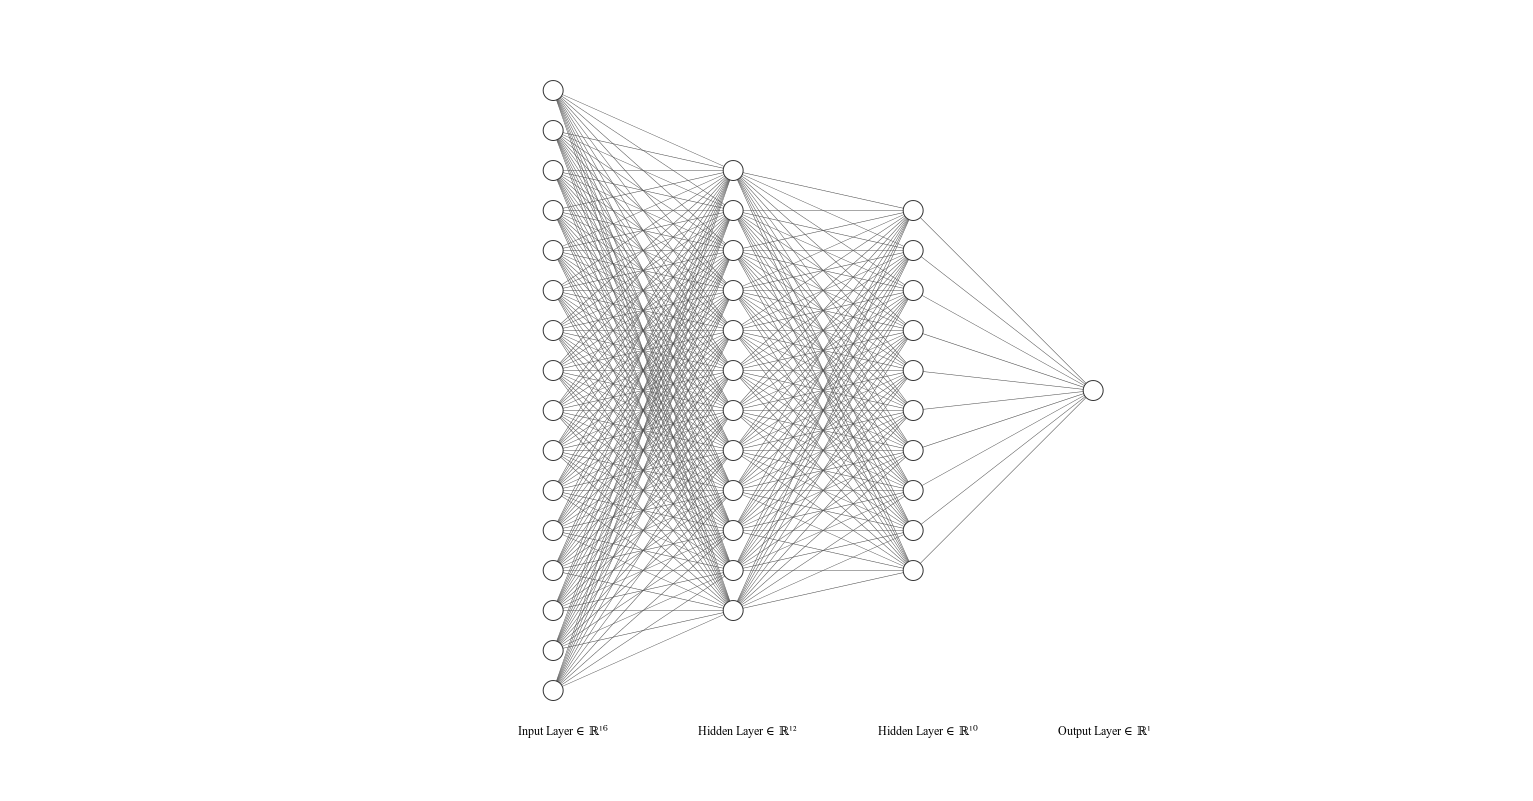
\includegraphics[keepaspectratio = true, scale=0.4,center]{img/nnExample.png}
	\caption{Esempio di rete neurale \textit{sequential}}
\end{figure}

\subsubsection{Struttura}
È stata scelto di utilizzare il tipo di rete \href{https://keras.io/getting-started/sequential-model-guide/}{\textit{Sequential}}.\\ 
Abbiamo creato due reti, con tre layer di tipo \href{https://keras.io/layers/core/}{\textit{Dense}}.
Le funzione di attivazione scelte sono le seguenti:
\begin{enumerate}
	\item \href{https://keras.io/activations/#relu}{\textit{Relu}} per i nodi interni;
	\item \href{https://keras.io/activations/#sigmoid}{\textit{Sigmoid}} per l'output della rete.
\end{enumerate}
La prima rete presenta la seguente struttura:
\begin{lstlisting}[backgroundcolor = \color{white}]
		model = Sequential([
        Dense(512, input_dim = num_max), 
        Activation('relu'),
        Dense(256), 
        Activation('relu'),
        Dense(1),
        Activation('sigmoid')
    ])
\end{lstlisting}


La seconda rete presenta la seguente struttura:
\begin{lstlisting}[backgroundcolor = \color{white}]
		model = Sequential([
        Dense(512, input_dim = num_max),
        Activation('relu'),
        Dropout(0.2),
        Dense(256),
        Activation('relu'),
        Dropout(0.2),
        Dense(1),
        Activation('sigmoid')
    ])
\end{lstlisting}


\subsubsection{Configurazione}
Tramite il metodo \textit{compile()} presente in Keras è possibile stabilire:
\begin{enumerate}
	\item \textbf{Loss functions}: \href{https://en.wikipedia.org/wiki/Cross_entropy}{\textit{binary crossentropy}} nel nostro caso, maggiori info al seguente link \href{https://keras.io/losses/}{\textit{loss functions}};
	\item \textbf{Optimizer}: l'ottimizzatore che verrà utilizzato per l'aggiustamento dei pesi e per minimizzare la loss function.
	Nel nostro caso \href{https://arxiv.org/pdf/1412.6980v8.pdf}{\textit{Adam}}. 
	\item \textbf{Metrics}: lista di metriche che verranno valutate dal modello durante la fase di training e testing.
	Nel nostro caso è stata scelta la metrica di \href{https://keras.io/metrics/#binary_accuracy}{\textit{binary accuracy}}.  
\end{enumerate} 
\subsection{Logistic Regression}
Il secondo approccio che abbiamo scelto di utilizzare è stato quello della logistic regression.
Per farlo ci siamo appoggiati alla libreria \href{https://scikit-learn.org/stable/}{\textit{Sklearn}}.
\subsubsection{Configurazione}
Tramite il metodo \textit{fit()} presente in Sklearn stabiliamo:
\begin{enumerate}
	\item \textbf{precision}: sono tutte quei messaggi classificati nel modo corretto, quindi attribuendogli la giusta etichetta. Maggiori informazioni al seguente link \href{https://scikit-learn.org/stable/modules/generated/sklearn.metrics.precision_score.html#sklearn.metrics.precision_score}{\textit{precision}};	
	\item \textbf{recall}: sono tutti quei messaggi classificati come non spam e che effetivamente fanno parte dei messaggi non spam. Nel nostro caso, maggiori informazioni al seguente link \href{https://scikit-learn.org/stable/modules/generated/sklearn.metrics.recall\_score.html#sklearn.metrics.recall\_score}{\textit{recall}};
	\item \textbf{f1}: viene calcolato tramite la media armonica di precisione e recupero. Nel nostro caso, maggiori informazioni al seguente link \href{https://scikit-learn.org/stable/modules/generated/sklearn.metrics.f1_score.html}{\textit{f1}}.  
\end{enumerate} 
